\subsection*{3.8 Gegeninduktion}
    \begin{minipage}{0.54\linewidth}
        \begin{empheq}[box = \fbox]{align*}
            U_{i2} &= L_{12} \frac{dI_1}{dt}\\
            L_{12} &= L_{21}
        \end{empheq}
        Übereinanderliegende Spulen gleicher Länge bzw. Fläche:\\
        \begin{empheq}[box = \fbox]{align*}
            L_{12} &= n_2 \frac{\Phi_1}{I_1} = \mu_0 n_1 n_2 \frac{A_1}{l_1}
        \end{empheq}
    \end{minipage}
    \begin{minipage}{0.44\linewidth}
        \begin{itemize}
            \item Feldspule$_1$: Spannung per Batterie
            \item Induktionsspule$_2$: Induzierte Spannung
        \end{itemize}
        \begin{scriptsize}
            \begin{empheq}{align*}
                U &= \text{el. Spannung}\\
                L &= \text{Induktivität}\\
                n &= \text{Windungen der Spule}\\
                \Phi &= \text{mag. Fluss durch Spule}\\
                A &= \text{Querschnittsfläche Spule}\\
                l &= \text{Länge Spule}\\
            \end{empheq}
        \end{scriptsize}
    \end{minipage}

    \subsubsection{Beispiel Transformator}
        \begin{minipage}{0.49\linewidth}
            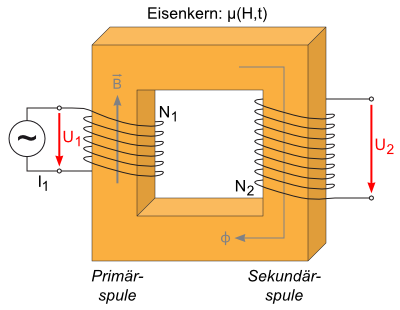
\includegraphics[width = \linewidth]{src/images/transformator.png}
        \end{minipage}
        \begin{minipage}{0.49\linewidth}
            \mathbox{\left| \frac{U_p}{U_s} \right| = \frac{n_p}{n_s}}
            \begin{scriptsize}
                \begin{align*}
                    p &= \text{Primärspule}\\
                    s &= \text{Sekundärspule}\\
                    U &= \text{el. Spannung}\\
                    n &= \text{Windungen}
                \end{align*}
            \end{scriptsize}
        \end{minipage}

    